\section{Methodology}\label{sec:methods}

Tran and Yates' \cite{tran2022dense} main contribution is to consider entities embeddings independently of the document or query embeddings obtained from pre-trained language model. To achieve this, they combine embeddings from pre-trained language model TAS BERT (Hofstätter et al. \cite{tasbert}) with Wikipedia2Vec (Yamada et. al \cite{yamada2018wikipedia2vec}) embeddings of entities extracted from documents and queries using. When combining with the document embeddings, the embeddings of entities provide multiple views on the same information, with different sets of entities representing various perspectives on the queries and documents. Depending on the displayed view, different relevant documents or sections of documents can be identified.

Tran and Yates do not use the information about documents and entities as an input for a learned framework, deviating from the cross-encoder approach (see \autoref{sec:introduction}). Instead, they merge these embeddings into a joint vector space. This joint vector space results in a final embedding used to calculate similarities between vectors. Thus, Tran and Yates adopt the bi-encoder model (as discussed in \autoref{sec:introduction}), allowing for indexing of document embeddings and enabling fast ranking computations through ANN search. 

\subsection{General Model}\label{subsec:general_model}

Tran and Yates' proposed method involves independent embeddings of documents and entities. The process entails merging the embeddings of both documents and entities for each query and document to achieve a joint vector space, as depicted in \autoref{fig:general_model}. Following the bi-encoder approach, the embeddings for queries and documents are created independently using the pre-trained language model TAS BERT (Hofstätter et al. \cite{tasbert}), which builds upon a distilled version of BERT (Sanh et al. \cite{sanh2019distilbert}).

\begin{figure}[!htb]
    \centering
    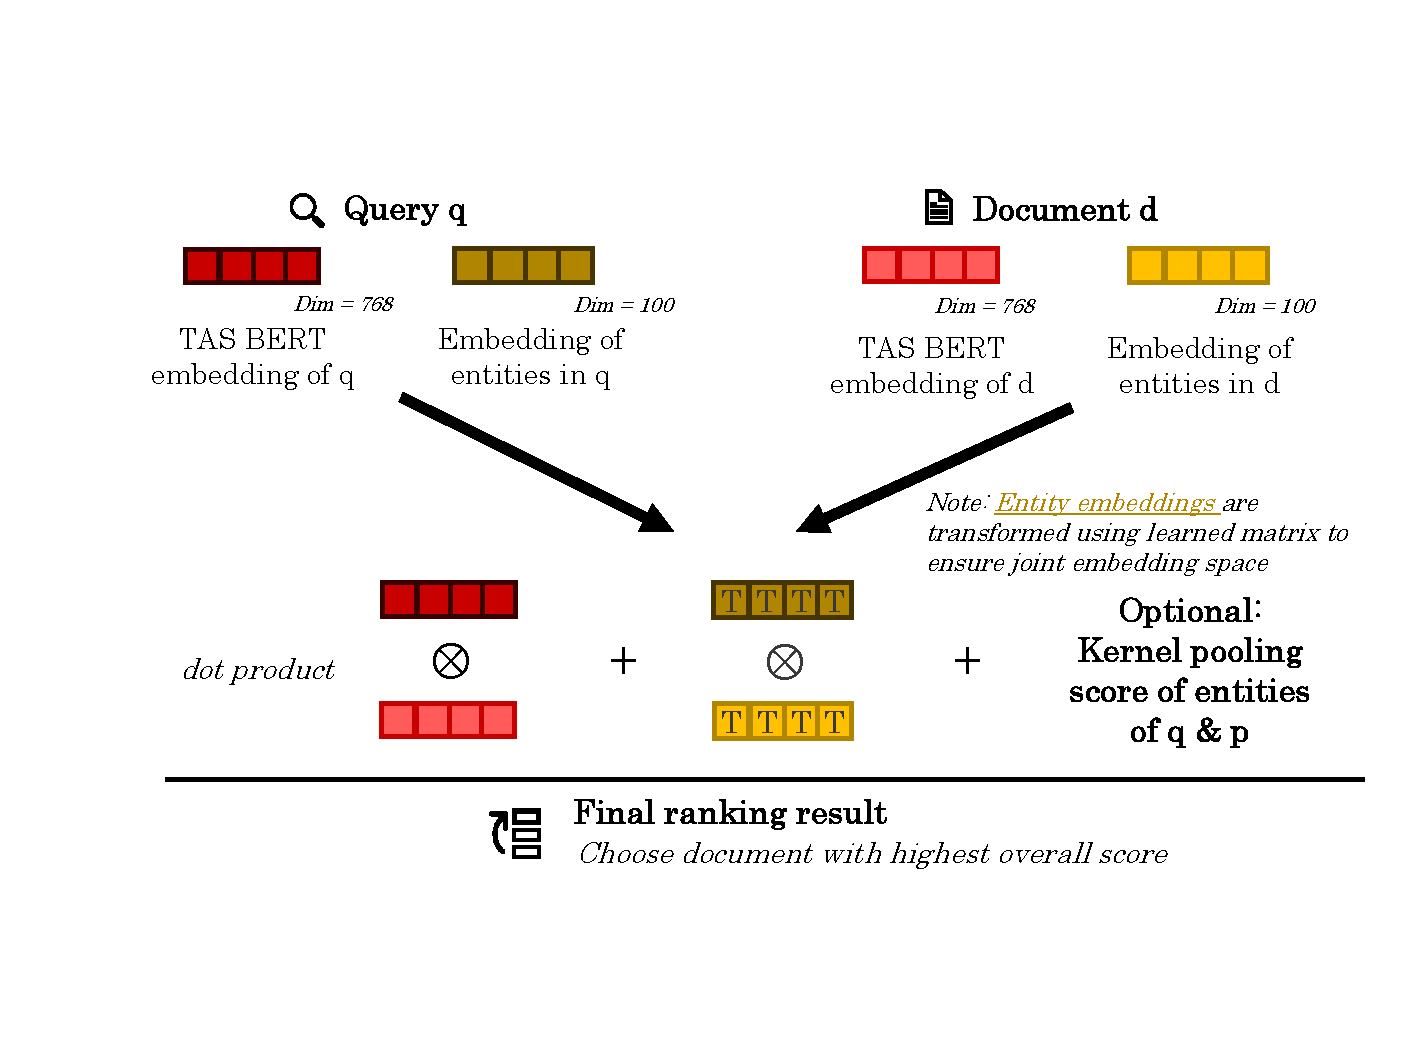
\includegraphics[trim={1.5cm 3.3cm 1.5cm 3.2cm}, clip, width=0.85\textwidth]{resources/general_model} 
    \caption{General model}
    \label{fig:general_model}
\end{figure}

The TAS BERT approach employs topic-aware sampling for fine-tuning on information retrieval task, thus queries in the training dataset are clustered based on different topics. During training, query samples are extracted exclusively from clusters with identical topics, aiming to enhance the sensitivity of the information retrieval model to different topics.

In the dense retrieval setting, embeddings of tokens are compared using similarity measurements to rank the best documents concerning a query. Tran and Yates follow a similar principle but enhance it by incorporating embeddings of entities. For each query and document, a single entity embedding is generated and concatenated with the textual embedding to create an embedding that captures both the semantic context and entity information. Final ranking is built upon dot product as similarity measurement.

Experimental results demonstrate that concatenation produces superior results for combining text and entity embeddings compared to other methods as max pooling and sum pooling. \autoref{tab:operator} displays the respective analysis of Tran and Yates based on their experimental setup, which is introduced in detail in \autoref{sec:results}. Apart from the analytical point of view, the approach of concatenation offers the advantage that it can be understood quite intuitively.

\begin{table}[!htb]
    \footnotesize
    \centering
    \begin{tabular}{llll}
    \hline
    \multirow{2}{*}{\textbf{Operators}} & \multicolumn{3}{c}{\textbf{MS Marco}}   \\
                                      & \textbf{nDCG} & \textbf{MRR} & \textbf{MAP} \\
    \hline
    Sum & 0.393 & 0.335 & 0.339 \\
    Max & 0.388 & 0.330 & 0.334 \\
    Concat & 0.396 & 0.341 & 0.343 \\
    \hline
    \end{tabular}
    \caption{Varying Aggregation Operators of Embedding Concatenation}
    \label{tab:operator}
\end{table}

However, concatenation introduces a challenge as the word embeddings and entity embeddings are generated in different vector spaces with varying dimensions and magnitudes. To address this issue, Tran and Yates introduce a transformation matrix $W \in \mathbb{R}^{100 \times 100}$ to transform the entity embeddings into the joint vector space. So let $\mathbf{E}(t) \in \mathbb{R}^{100}$ be the embedding of entities of text $t$, the transformed entity embedding is given as:
\begin{align}
    \mathbf{R}_{entity}(t) = W^T \cdot \mathbf{E}(t)
\end{align}
The values of the matrix are determined during training process and thus reflect a meaningful transformation of the embeddings into a joint vector space. 

Given a text $t$ with its corresponding word embedding $\mathbf{R}_{text}(t)$ derived from the pre-trained language model, the final vector representation of $t$ is obtained by concatenating the transformed entity embedding $\mathbf{R}_{entity}(t)$ and the word embedding:
\begin{align}
\mathbf{R}_{final}(t) &= \mathbf{R}_{text}(t) \oplus \mathbf{R}_{entity}(t)
\end{align}
The ranking score value of a pair of query $q$ and document $d$ is then obtained using the dot product $\otimes$ as a similarity measure:
\begin{align}
    \mathbf{Score}(q,d) &= \left( \mathbf{R}_{final}(q) \otimes \mathbf{R}_{final}(d) \right) \\
    &= \left( \mathbf{R}_{text}(q) \otimes \mathbf{R}_{text}(d) \right) \oplus \left( \mathbf{R}_{entity}(q) \otimes \mathbf{R}_{entity}(d) \right)
\end{align}
As an optional addition to their model, Tran and Yates include a kernel based neural ranking model (KNRM, Xiong et al. \cite{xiong2017end}) as an external scoring source, which predicts the similarity between document and query entities. This interaction-based approach requires knowledge of the query and document at runtime. For details, refer section \ref{subsec:knrm}. Incorporating the KNRM signal $S_{knrm}$ into the final ranking score yields the score with KNRM signal, denoted by $\mathbf{Score}_{knrm}(q,d)$:
\begin{align}
    \mathbf{Score}_{knrm}(q,d) &= \left( \mathbf{R}_{final}(q) \otimes \mathbf{R}_{final}(d) \right) + S_{knrm} \label{eq:score_knrm}
\end{align}
\subsection{Generating Entity Embeddings\label{subsec:entity_embeddings}}
As described in section \ref{subsec:general_model}, Tran and Yates create embeddings for both text and entities in queries and documents. While the text embeddings are generated using TAS BERT, the primary focus of the contribution of Tran and Yates lies in the creation of entity embeddings. In particular, as queries and documents often contain multiple entities, these entities need to be aggregated into a single embedding.

To illustrate this process, consider the example in \autoref{fig:example}. In this example, the query 'Favourite book bert sesame street' corresponds to a document that mentions three entities: Bert, Sesame Street and Boring Stories.

\begin{figure}[!htb]
    \centering
    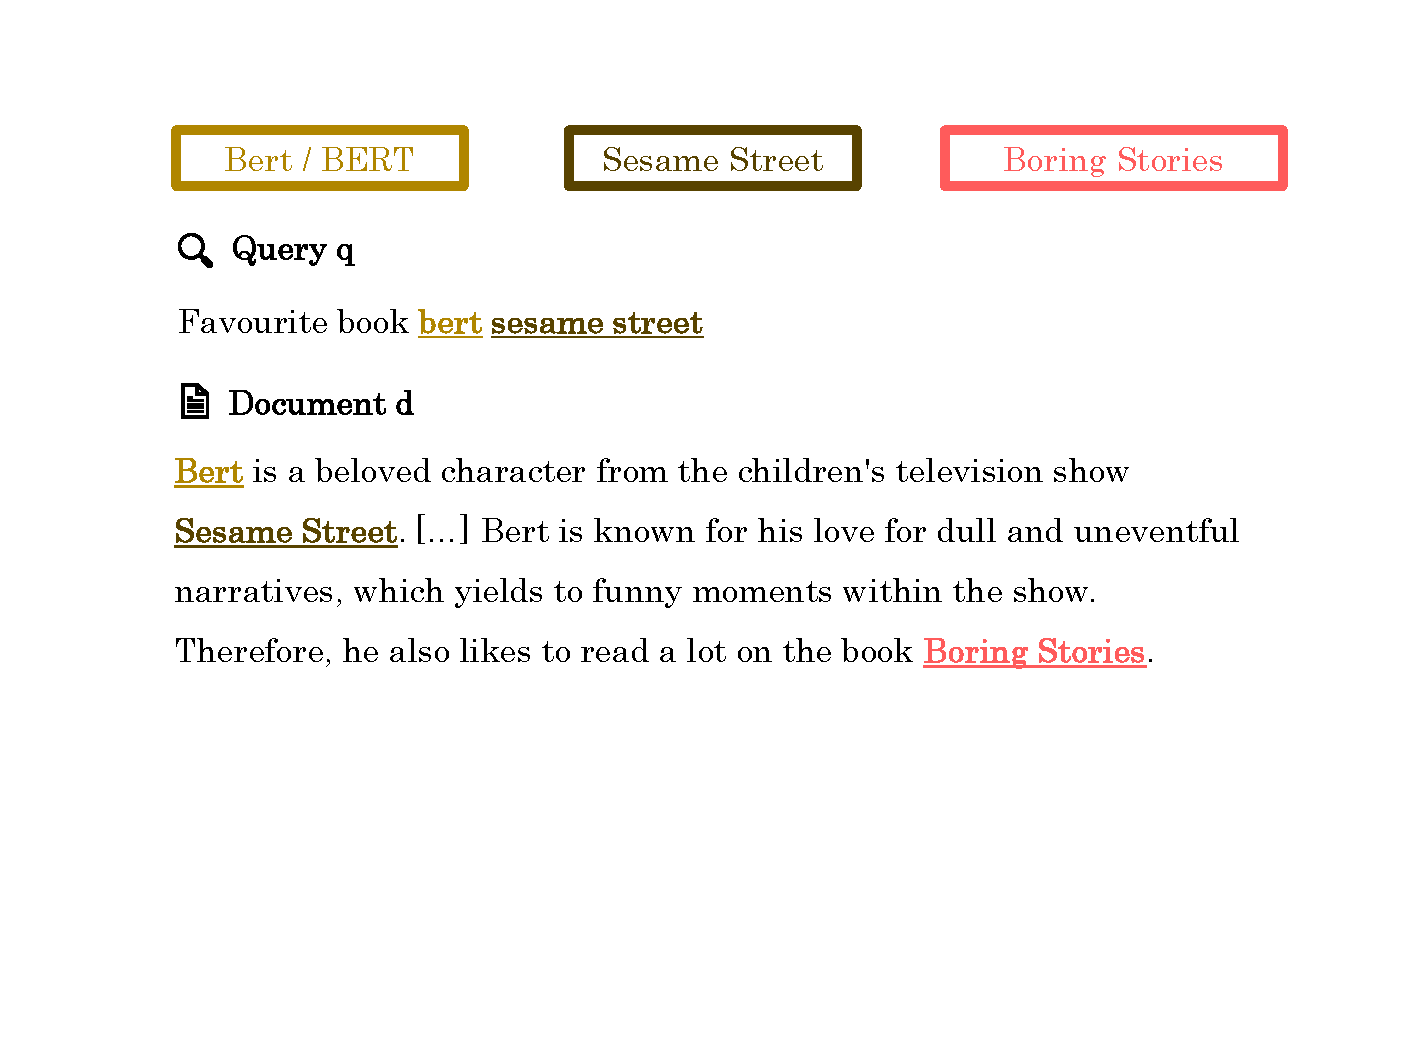
\includegraphics[trim={1.5cm 6.7cm 1.5cm 2cm}, clip, width=0.9\textwidth]{resources/example_2} 
    \caption{Example query and example document}
    \label{fig:example}
\end{figure}

\subsubsection{Extracting Entities}\label{subsubsec:extracting_entities}

To aggregate multiple entities in a document or query, Tran and Yates first extract these entities from the text using external frameworks Dexter (Ceccarelli et al. \cite{ceccarelli2013dexter}) and Wikipedia2Vec (Yamada et. al \cite{yamada2018wikipedia2vec}).
\begin{itemize}
    \item The Dexter framework is an entity linkage system that resolves entity mentions in text to corresponding entities in a knowledge base. In particular, Dexter employs a combination of methods, including named entity recognition and pattern matching, to perform this task. 
    \item Wikipedia2Vec leverages the structure of Wikipedia to generate dense vector representations (embeddings) for words, articles, and entities. It utilizes the Word2Vec algorithm (Mikolov et al. \cite{mikolov2013distributed}) to capture semantic relationships from Wikipedia, producing high-dimensional embeddings.
\end{itemize}

\begin{figure}[!htb]
    \centering
    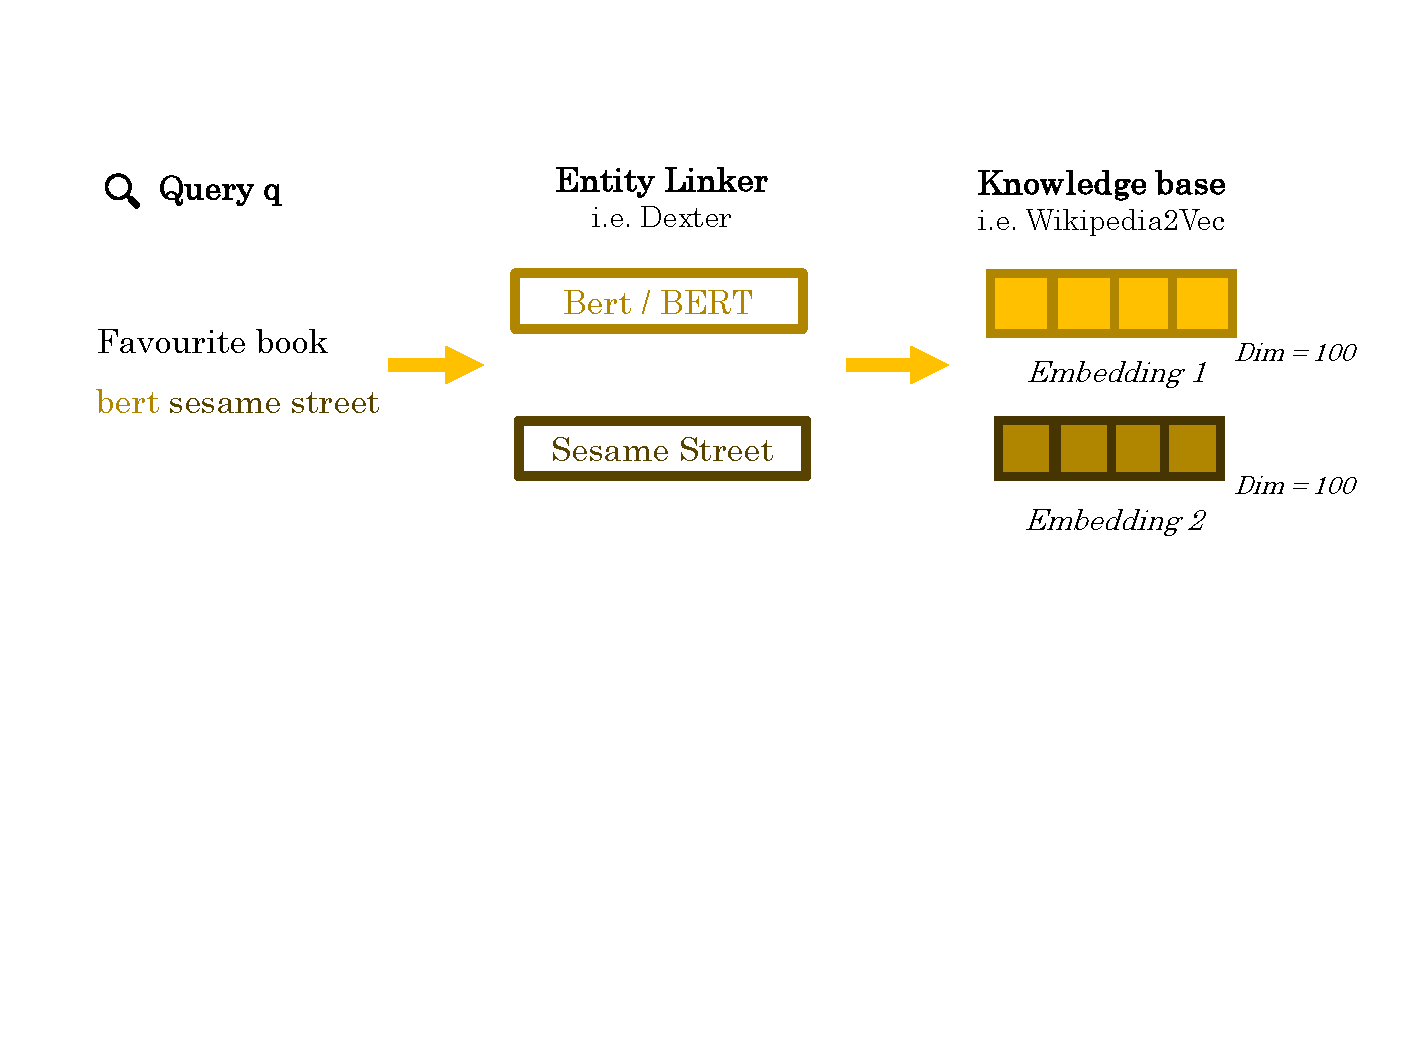
\includegraphics[trim={1cm 9cm 1cm 2.5cm}, clip, width=0.85\textwidth]{resources/entity_extraction_2} 
    \caption{Process of entity extraction}
    \label{fig:entity_extraction}
\end{figure}

The extraction procedure involves submitting a document or query to Dexter, which extracts entity mentions from the given text. These entity names are then passed on to the knowledge base, which transforms them into embeddings. Wikipedia2Vec provides vectors in dimension 100 as default. Tran and Yates keep this value and therefore generate entity embeddings in dimension 100. \autoref{fig:entity_extraction} visualizes this process.


\subsubsection{Combining Entities for Queries}\label{subsub:generating_queries}

For now, multiple embeddings for each entity within a query or a document are generated by applying the procedure outlined in section \ref{subsubsec:extracting_entities}. The aggregation of these generated embeddings differs based on whether a query or a document is considered, given the usual brevity of queries compared to documents.

For queries, Tran and Yates adopt a straightforward approach. They aggregate the embeddings of entities by averaging all entity embeddings across all dimensions. \autoref{fig:queries} visualizes this procedure.

\begin{figure}[!htb]
    \centering
    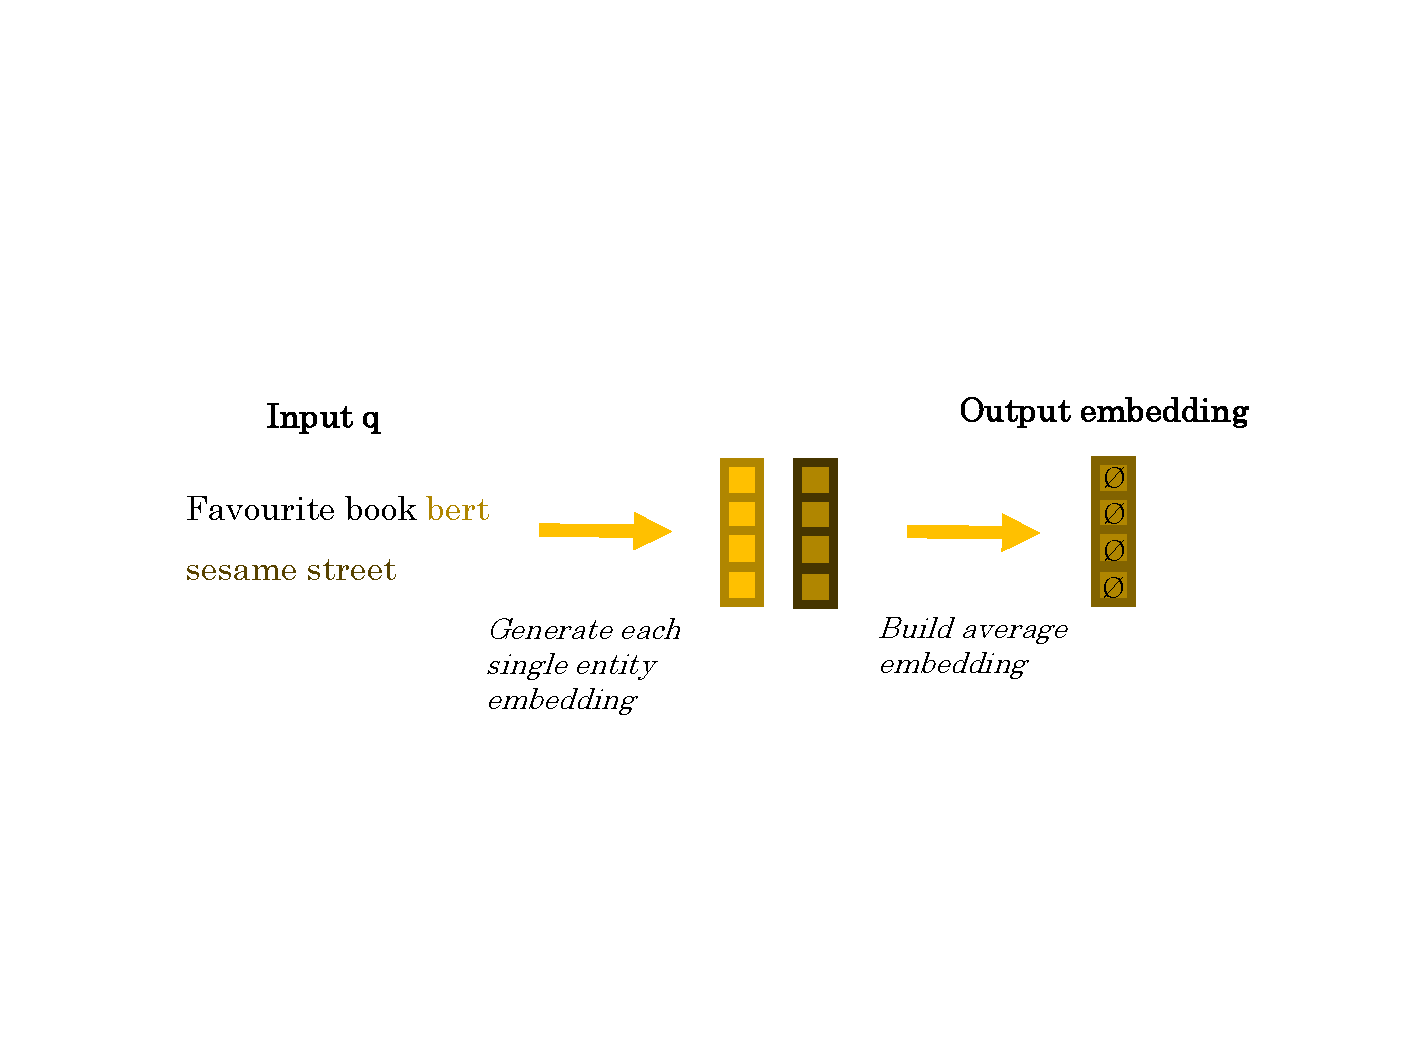
\includegraphics[trim={2cm 5.9cm 2cm 6.5cm}, clip, width=0.8\textwidth]{resources/queries} 
    \caption{Process of generating a single entity embedding for a query}
    \label{fig:queries}
\end{figure}

\subsubsection{Combining Entities for Documents}\label{subsec:models}

Documents usually contain many different entities, as the example in \autoref{fig:example} indicates. Additionally, documents might also cover different aspects of a topic, so entities from very different areas might appear within them. To handle this additional complexity, the authors proposed three successive methods for entity aggregation in documents, namely:

\begin{itemize}
    \item Single Entity Representation (EVA Single)
    \item Query-Aware Single Entity Representation (EVA Single-QA)
    \item Multiple Entity View Representation (EVA Multi)
\end{itemize}

The term 'EVA' stands for \underline{E}ntity \underline{V}iews in Dense Retriev\underline{a}l. The concept of 'Entity Views' which gives the paper its name, is particularly relevant in the third method, EVA Multi, and will be elaborated in the following sections.

\paragraph*{EVA Single}

The initial approach for aggregating entities in a document, called EVA Single, is similar to the one used for queries. The key idea behind the Single Entity Representation is to extract all entities present in the document and subsequently generate a single output embedding by computing the average of these entity embeddings. This process is analogous to the one depicted in \autoref{fig:queries} for queries, and a visual representation for documents is illustrated in \autoref{fig:eva_single}.

\begin{figure}[!htb]
    \centering
    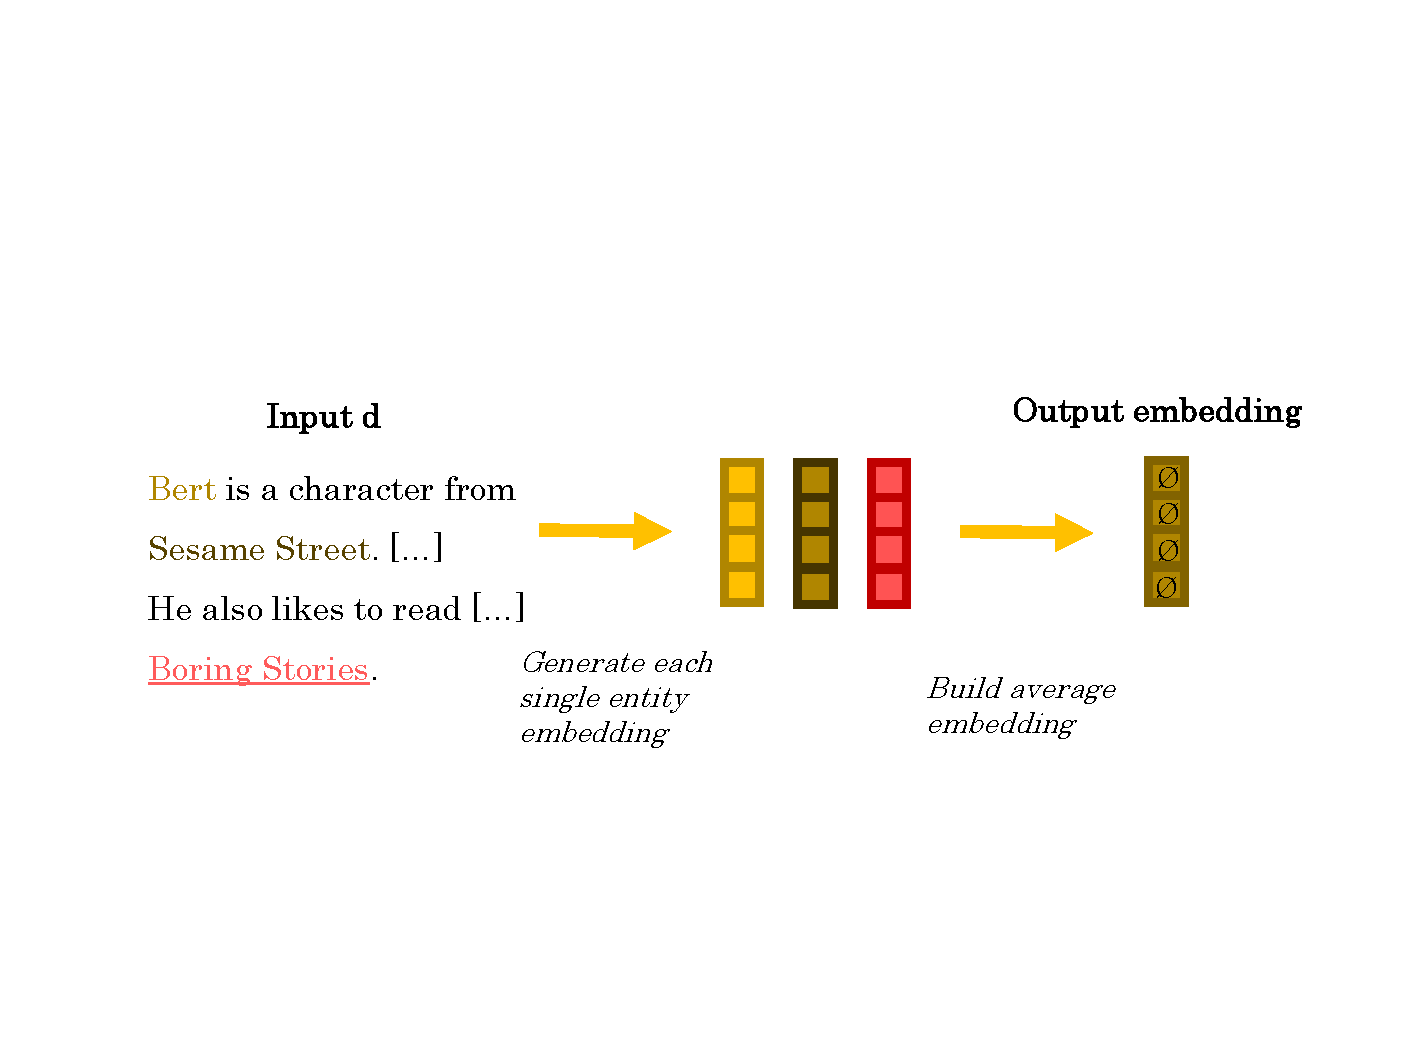
\includegraphics[trim={2cm 5cm 1.5cm 6.5cm}, clip, width=0.8\textwidth]{resources/eva_single} 
    \caption{Process of generating an entity embedding for a document following the EVA Single approach}
    \label{fig:eva_single}
\end{figure}

Despite its simplicity, this approach overlooks the fact that documents may cover diverse topics. By discarding query information, the EVA Single approach considers all entities, including those that may be only partially relevant to the document's main topic. Consequently, this disregards the relevance of entities within the ranking process, leading to biased results, as observed in \autoref{sec:results}.

\paragraph*{EVA Single-QA}

To address the problem of EVA Single disregarding the entities of queries, Tran and Yates introduce the Query-Aware Single Entity Representation. This approach creates embeddings that are tailored to the specific needs of a given query. However, this improvement comes with increased computational complexity since it assumes knowledge of the query beforehand. As a result, calculations for all query-document pairs must be performed during runtime, eliminating the possibility of precomputing document embeddings and indexing, leading to higher query latency, as observed in \autoref{sec:results}.

The underlying idea of the EVA Single-QA model is to filter the entities of a document based on the information of a given query and select only entities with high similarity to a query entity. \autoref{fig:eva_single_qa} visualizes this process.

\begin{figure}[!htb]
    \centering
    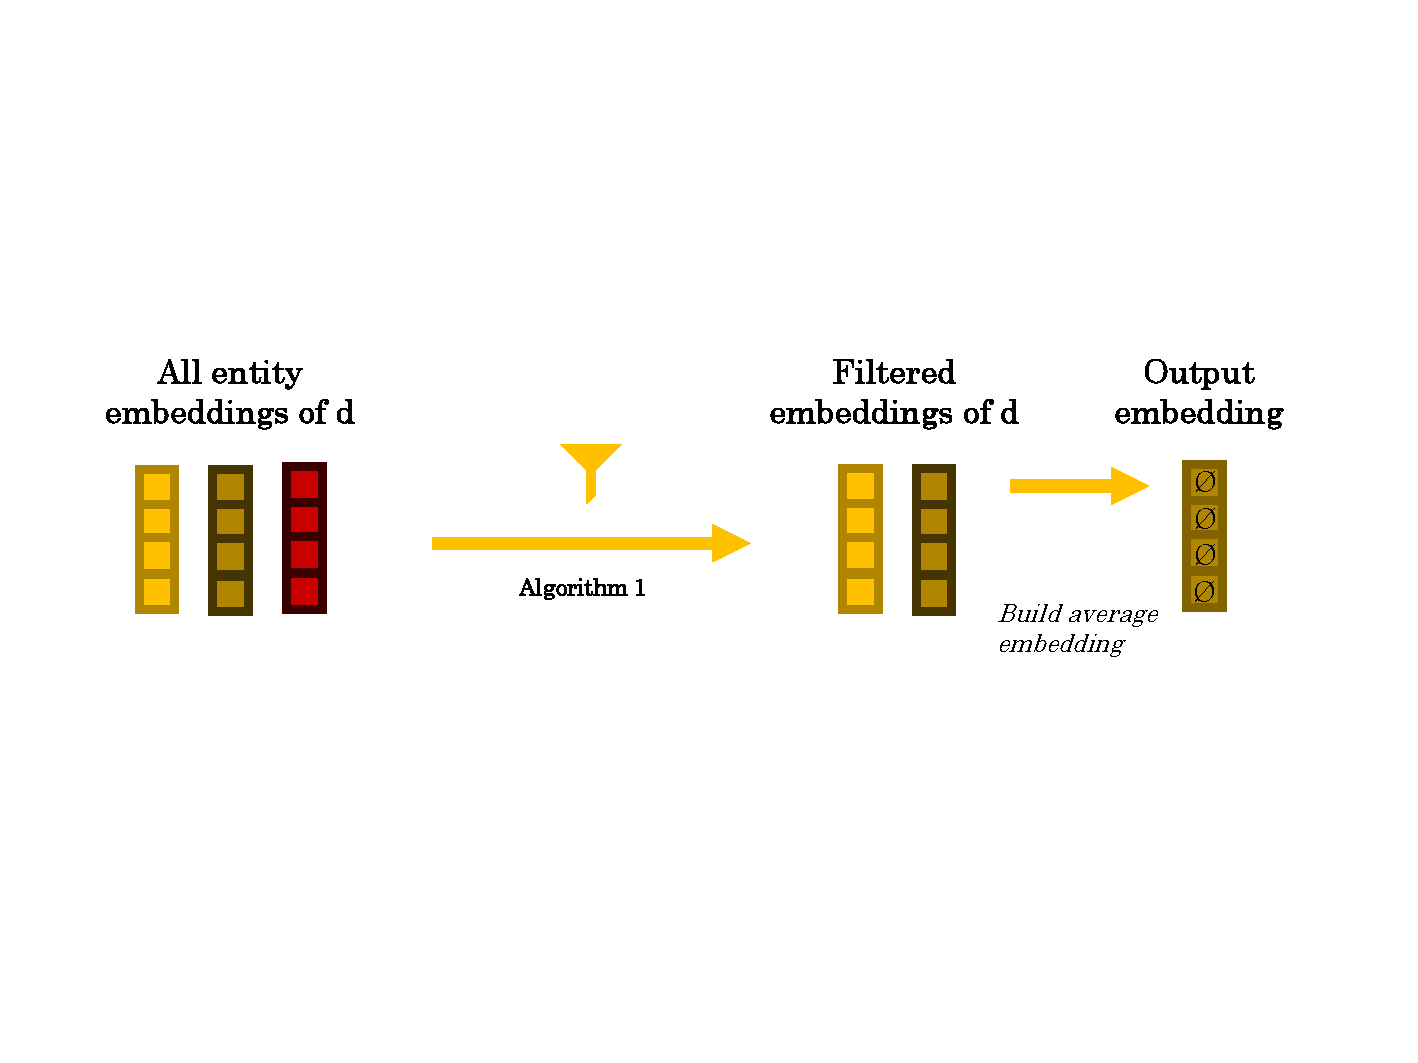
\includegraphics[trim={1cm 6.5cm 2cm 6cm}, clip, width=0.8\textwidth]{resources/eva_single_qa} 
    \caption{Process of generating an entity embedding for a document following the EVA Single-QA approach}
    \label{fig:eva_single_qa}
\end{figure}

The filtering is conducted using Algorithm \ref{alg:query-aware-entity-representation}, which is applied to each query-document pair ($q$, $d$). For every entity within $q$, the algorithm searches for the corresponding entity in $d$ that possesses the maximum cosine similarity. If the similarity exceeds a specified threshold $\alpha$, the respective entity in $d$ is added to the filtered list $X_{focus}(d)$. Subsequently, the single output embedding for document $d$ is computed as the average of all entity embeddings within $X_{focus}(d)$.

\begin{algorithm}[!htb]
    \footnotesize
    \caption{Query-aware document entity representation}
    \label{alg:query-aware-entity-representation}
    \begin{algorithmic}[1]
    \REQUIRE Query $q$ and document $d$, threshold $\alpha$
    \ENSURE Filtered entity embedding list $X_{focus}(d)$ of $d$
    
    \STATE $X(q) \leftarrow$ set of embeddings of entities in $q$
    \STATE $X_{focus}(d) \leftarrow \{\}$
    \FOR{$e$ in $X(q)$}
        \STATE $e^* \leftarrow$ entity embedding in $d$ having the maximum cosine similarity with $e$
        \IF{cosine similarity$(e^*, e) > \alpha$}
            \STATE $X_{focus}(d) \leftarrow X_{focus}(d) \cup \{e^*\}$
        \ENDIF
    \ENDFOR
    \RETURN $X_{focus}(d)$
    \end{algorithmic}
\end{algorithm}

\paragraph*{EVA Multi}

To address the issue of known queries required by the EVA Single-QA approach, Tran and Yates propose the EVA Multi method, which introduces multiple entity views as a solution with minimal negative consequences.

Analysis of training data revealed that in the vast majority of instances, the number of entities in queries does not exceed two. As shown in \autoref{tab:query_statistics}, in the MS MARCO dataset, 99.6 \% of the 300,000 training instances and 99.5 \% of the test instances contain two or fewer entities. Based on this observation, Tran and Yates focused their research on the assumption that it is sufficient to consider a maximum of two entities in queries.

\begin{table}[!htb]
    \centering
    \footnotesize
    \begin{tabular}{lp{2cm}cp{2cm}c}
    \hline
    \multirow{2}{*}{\textbf{Entities}} & \multicolumn{2}{c}{\textbf{Training Queries}} & \multicolumn{2}{c}{\textbf{Testing Queries}} \\
                                 & \textbf{Count}           & \textbf{Fraction}          & \textbf{Count}           & \textbf{Fraction}          \\
    \hline
    0 & 130,353 & 0.435 & 3,442 & 0.483 \\
    1 & 149,073 & 0.497 & 3,232 & 0.454 \\
    2 & 19,207 & 0.064 & 416 & 0.058 \\
    3+ & 1,367 & 0.004 & 37 & 0.005 \\
    \hline
    \textbf{Total} & 300,000 &  & 7,127 &  \\
    \textbf{Average} & 0.640 &  & 0.587 &  \\
    \hline
    \end{tabular}
    \caption{Summary statistics of queries}
    \label{tab:query_statistics}
\end{table}

Under this assumption, when applying Algorithm \ref{alg:query-aware-entity-representation}, at most two entities remain in the filtered embedding list $X_{focus}$. This limitation stems from the algorithm iterating over the set of all entities in the given query once, resulting in $X_{focus}$ containing either zero, one, or at most two items. Therefore, the number of all possible sets eligible for $X_{focus}$ is bounded.

Leveraging this observation, Tran and Yates introduce clusters of entities, which represent different views of a document. In the EVA Multi approach, all possible single itemsets and sets of pairs of the entities are generated, yielding set $clusters$. However, sets of pairs are considered only if the cosine similarity between the two entities within a pair exceeds a predefined threshold $\beta$, ensuring only relevant entity views are generated. Subsequent algorithm \ref{alg:clusters} carries out this procedure.


\begin{algorithm}[!htb]
    \footnotesize
    \caption{Multiple cluster sets of document}
    \label{alg:clusters}
    \begin{algorithmic}[1]
    \REQUIRE Document $d$, maximum cluster size $M$ (= 2)
    \ENSURE Multiple cluster total representations of $d$
    \STATE $X(d) \leftarrow$ set of all entities in $p$
    \STATE $clusters \leftarrow \emptyset$
    \FOR {every non-empty subset $C \subset X(d)$ with size $l \leq M$}
        \IF {$l = 1$ or (every pair of entities in $C$ has cosine similarity $> \beta$)}
            \STATE $clusters \leftarrow clusters \cup C$
        \ENDIF
    \ENDFOR
    \RETURN $clusters$
    \end{algorithmic}
\end{algorithm}

The final output embeddings are then calculated by averaging the embeddings of all items within each set in $clusters$. When applying the optional KNRM signal (see section \ref{subsec:knrm}) to this approach, the entity interaction matrix $T$ is built only upon the set of entity embeddings within a single cluster, rather than considering all entities within the document.

\begin{figure}[!htb]
    \centering
    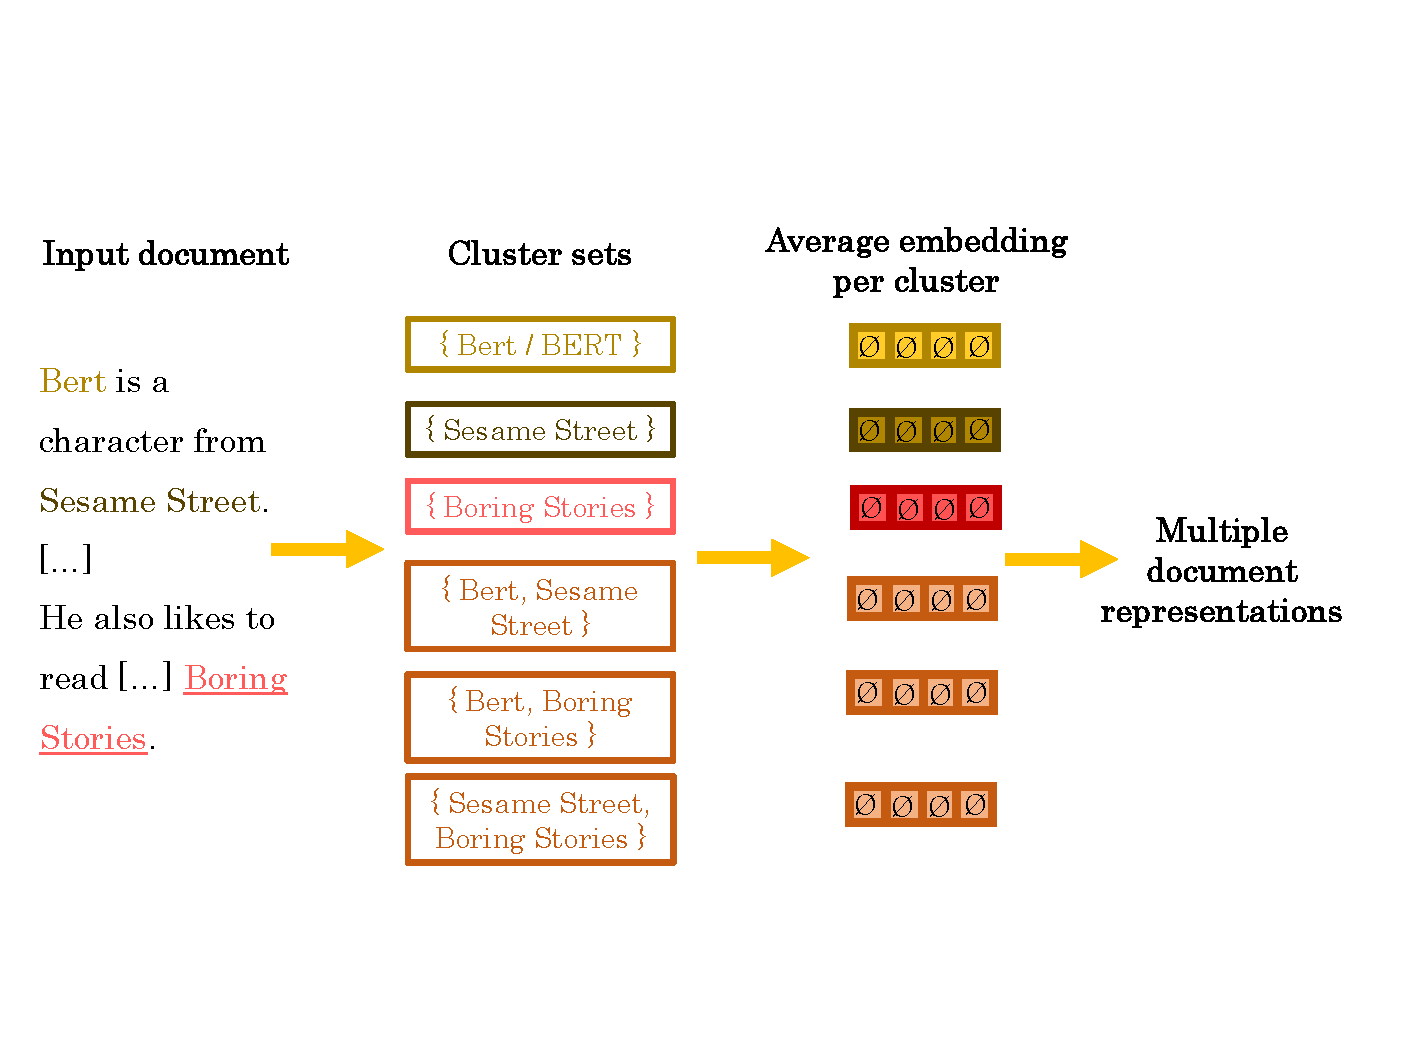
\includegraphics[trim={0cm 3.4cm 0cm 3.8cm}, clip, width=\textwidth]{resources/eva_multi} 
    \caption{Process of generating entity embeddings for a document following the EVA Multi approach}
    \label{fig:eva_multi}
\end{figure}

This allows all calculations to be performed independently of query information, enabling indexing. Unlike the previous methods, EVA Single and EVA Single-QA, the EVA Multi approach generates several entity output embeddings per document. \autoref{fig:eva_multi} visualizes the process of generating the embeddings of multiple entity views or clusters.

\subsection{KNRM Signal}\label{subsec:knrm}

Tran and Yates introduce a kernel based neural ranking model (KNRM), originally developed by Xiong et al. \cite{xiong2017end}, as an additional scoring mechanism to extend their approach of incorporating entity embeddings into bi-encoder model. Unlike its original use, Tran and Yates adapt the KNRM model to specifically capture the interaction between entities in queries and documents. \autoref{eq:score_knrm} depicts the integration of the KNRM signal $S_{knrm}$ into the calculations for the final ranking score, which Tran and Yates apply for the EVA Single-QA and EVA Multi models, yielding in EVA Single-QA-KNRM and EVA Multi KNRM models (see \autoref{sec:results}). 

The calculation of the KNRM signal follows these steps:

\begin{enumerate}
    \item Let $X(q)$ be the set of all entity embeddings within query $q$, $X(d)$ any set of entity embeddings which occur in document $d$. For EVA Single and EVA Single-QA models (see section \ref{subsec:models}) $X(d)$ contains all entities with the given document, for EVA Multi (see section \ref{subsec:models}) $X(d)$ contains only entities of specific subsets of entities of $d$. The entity interaction matrix is defined as:
    \[T_{i,j} := sim(X_i(q), X_j(d)) \text{~,}\] 
    where $X_i(q)$ and $X_j(d)$ are the $i$-th and $j$-th entity embedding of $q$ and $d$. The similarity function is given as cosine similarity. Embeddings are generated via Wikipedia2Vec (Yamada et. al \cite{yamada2018wikipedia2vec}), as described in section \ref{subsubsec:extracting_entities}.
    \item Build k kernels using radial basis function, which creates differentiable histograms around hyperparameters $\mu_i$ and $\sigma^2_i$ for $i \in \{1, \dots, |X(q)|\}$.
    \[ K_l(X_i(q)) = \sum_{j=1}^{|X(p)|}\exp\left(-\frac{(T_{i,j}-\mu_i)^2}{2\sigma_i^2}\right)\]
    \item Pool / Summarize the k results into a k-dimensional feature vector: \[\overrightarrow{K(X_i(q))} = [K_1(X_i(q)), \ldots, K_k(X_i(q))]\]
    \item Build kernel-pooled representation $\phi(T)$ by calculating log-sum for each query entity: \vspace{-0.5cm}\[\phi(T) = \sum_{i=1}^{|X(q)|} \log \overrightarrow{K(X_i(q))}\vspace{-0.3cm}\]
    \item Get final kernel pooling score by applying a learned ranking layer. Note that $\tanh(\cdot) \in (-1, 1)$ and therefore $\sup S_{knrm} = 1$: \[ S_{\text{knrm}} = \tanh(w^T\phi(T) + b) \vspace{-0.3cm}\]
  \end{enumerate}

Despite being an interaction-based model that requires scoring during runtime for all query-document pairs, the computational complexity of the KNRM approach remains limited. The computations involved are relatively straightforward, and the additional learned layer does not significantly increase the computational overhead. Furthermore, these computations can be performed in parallel with the other components of Tran and Yates' approach. Empirical results concerning the latency of the models, with and without the KNRM signal, validate this assertion (see \autoref{sec:results}).



